\section{Exact Solution: Geometric Representation}
\label{subsec:qubit_exact_geometry}

We now put the machinery of Secs.~\ref{sec:generating_function}--\ref{sec:qubit_closure} to work
in the transverse-coupling spin-boson model. The qubit is the prototypical rank-1 case of the general framework, yet its $\mathfrak{su}(2)$ algebra is rich enough to generate all the essential non-perturbative physics. As illustrated in Fig.~\ref{fig:bloch_overview}, the exact qubit mean-force state $\mathbf{r}$ lives in a three-dimensional Bloch sphere, but is geometrically locked to the \emph{coupling plane} (shaded) spanned by the system axis $\hat{\mathbf{n}}_s$ and the interaction axis $\hat{\mathbf{f}}$. The orientation of this plane is defined by the interaction phase $\phi_f$, which directly determines the phase of the induced coherences in the reduced state. 

We first define our system Hamiltonian and coupling via
\begin{equation}
    H_Q = \frac{\omega_q}{2} \hat{\mathbf{n}}_s \cdot \boldsymbol{\sigma}, \qquad f = \hat{\mathbf{f}} \cdot \boldsymbol{\sigma},
\end{equation}
where $\hat{\mathbf{n}}_s$ and $\hat{\mathbf{f}}$ are unit vectors defining the system and coupling axes, respectively.
 The overall coupling strength $g$ is omitted in the following derivation for clarity and can be re-introduced as a global scaling factor where needed.
For the derivation it is convenient to work in the eigenbasis of $H_Q$ (so
$\hat{\mathbf{n}}_s=\hat{\mathbf z}$). The final formulas are then rewritten
covariantly in terms of $\hat{\mathbf{n}}_s$ and $\hat{\mathbf{f}}_\perp$.

\begin{figure}[t]
    \centering
    
\includegraphics[width=\columnwidth]{../figures/hmf_bloch_3d_overview.pdf}
    \caption{3D geometric overview of the exact qubit mean-force state. The system is defined by the bare axis $\hat{\mathbf{n}}_s$ and the interaction axis $\hat{\mathbf{f}}$ at polar angle $\theta$ and azimuthal angle $\phi_f$. The exact reduced-state Bloch vector $\mathbf r$ is constrained to the shaded coupling plane. The interaction phase $\phi_f$ rotates the coupling plane and sets the phase of the steady-state coherences.}
    \label{fig:bloch_overview}
\end{figure}



The influence exponent may easily be calculated directly, using $\tilde f(\tau)=e^{\tau H_Q} f e^{-\tau H_Q}$. In the qubit energy basis ($\hat{\mathbf{n}}_s = \hat{\mathbf{z}}$), we decompose the unit coupling vector as $\hat{\mathbf{f}} = (s \cos\phi_f, s \sin\phi_f, c)$, where $c \equiv \cos\theta$ and $s \equiv \sin\theta$ denote the longitudinal and transverse projections relative to the system axis, and $\phi_f$ is the azimuthal angle. Writing
\begin{equation}
\begin{split}
    f &= c\sigma_z + f_-\sigma_+ + f_+\sigma_-, \\
    f_\pm &\equiv s e^{\pm i \phi_f},
\end{split}
\end{equation}
gives
\begin{equation}
    \tilde f(\tau)=c\sigma_z+f_-e^{\omega_q\tau}\sigma_+ + f_+e^{-\omega_q\tau}\sigma_-,
\end{equation}
meaning $\Delta(\beta)$ is determined solely by the bath response kernels at the frequencies $0,\pm\omega_q$. Consequently,
all bath dependence in $\Delta$ is compressed to scalar kernel data evaluated
at the same frequencies. Using the notation of
Sec.~\ref{subsec:kms_symmetry}, the required bath objects are
$\mathcal{K}(0)$, $\mathcal{K}(\pm\omega_q)$, and $R(0)$,
$R(\pm\omega_q)$. 



For a single qubit, the operator algebra closes almost trivially. Using $\sigma_+\sigma_-=(\mathbb
I+\sigma_z)/2$, $\sigma_-\sigma_+=(\mathbb I-\sigma_z)/2$, and
$\sigma_\pm^2=0$, one finds
\begin{equation}
\begin{aligned}
    \tilde{f}(\tau)\tilde{f}(\tau')
    &= \Big[c^2 + s^2\cosh\big(\omega_q(\tau-\tau')\big)\Big]\mathbb{I} \\
    &\quad + s^2\sinh\big(\omega_q(\tau-\tau')\big)\sigma_z \\
    &\quad + c f_- \left(e^{\omega_q\tau'} - e^{\omega_q\tau}\right)\sigma_+ \\
    &\quad + c f_+ \left(e^{-\omega_q\tau} - e^{-\omega_q\tau'}\right)\sigma_- .
\end{aligned}
\end{equation}

Using the response kernels, the entirety of the bath's influence is compressed into two real, temperature-dependent response kernels: a longitudinal (resonant) kernel $\Sigma_z$ and a transverse (non-resonant) kernel $\Sigma_{\perp}$, defined as
\begin{equation}
    \Sigma_z \equiv \frac{1}{2} \left[R(\omega_q) - R(-\omega_q)\right], \quad \Sigma_\perp \equiv \frac{4}{\omega_q} \left[ \cosh\left(\frac{\beta\omega_q}{2}\right) \mathcal{K}(0) - e^{-\beta\omega_q/2} \mathcal{K}(\omega_q) \right].
    \label{eq:bath_kernels_direct}
\end{equation}
After performing the non-perturbative recombination (with the algebraic derivation detailed in Appendix~\ref{app:qubit_ladder_derivation}), the exact reduced density matrix $\rho_Q$ takes the form:
\begin{equation}
    \rho_Q = \frac{1}{2} \begin{pmatrix} 
        1 + \tanh\Theta & \kappa \operatorname{sech}\Theta e^{-i\phi_f} \\
        \kappa \operatorname{sech}\Theta e^{i\phi_f} & 1 - \tanh\Theta
    \end{pmatrix}.
    \label{eq:rho_matrix_general}
\end{equation}
The operant parameters here --- the renormalised thermal scale $\Theta$ and coherence strength $\kappa$ --- are given by
\begin{equation}
    \Theta \equiv \operatorname{arctanh}(\gamma s^2 \Sigma_z) - \frac{\beta\omega_q}{2},
    \qquad
    \kappa \equiv \frac{-\gamma c s \Sigma_\perp}{\sqrt{1 - (\gamma s^2 \Sigma_z)^2}},
\end{equation}
where $\gamma = \tanh\chi/\chi$ is the non-perturbative resummation factor determined by the influence magnitude $\chi \equiv |\mathbf h_{\mathrm{eff}}|$. Vectorially, the traceless symmetrised influence is $M = \mathbf h_{\mathrm{eff}} \cdot \boldsymbol{\sigma}$ with
\begin{equation}
    \mathbf h_{\mathrm{eff}} = \left( - \Sigma_\perp c s \cos\phi_f, - \Sigma_\perp c s \sin\phi_f, \Sigma_z s^2 \right),
    \label{eq:heff_def}
\end{equation}
such that the crossover parameter factorises as
\begin{equation}
    \chi = s \sqrt{s^2 \Sigma_z^2 + c^2 \Sigma_\perp^2} \equiv g^2 \chi_0(\beta, \theta).
    \label{eq:chi_factored}
\end{equation}
This representation reveals the reduced state $\rho_Q$ as dependent on a renormalised thermal scale set by $\Theta$, with its coherence dependent on the off-resonant bath response via $\kappa$. 

From this matrix representation, we may directly identify the correspondence between the interaction geometry and the reduced state. The diagonal elements $\rho_{00}, \rho_{11}$ determine the longitudinal population along $\hat{\mathbf{n}}_s$, while the off-diagonal elements $\rho_{01}, \rho_{10}$ capture the coherences. Crucially, the phase of the coupling $e^{\pm i \phi_f}$ (the azimuthal orientation of $\hat{\mathbf{f}}$) is perfectly preserved in the state coherences, up to a sign $\operatorname{sgn}(\kappa)$. In terms of the Bloch vector $\mathbf{r} = (r_x, r_y, r_z)$, the steady-state is
\begin{equation}
    r_z = \tanh\Theta, \qquad r_\perp = |\kappa \operatorname{sech}\Theta|, \qquad \phi_r = \phi_f + \pi \mathcal{H}(\Sigma_\perp c),
    \label{eq:bloch_components}
\end{equation}
where $r_\perp$ denotes the transverse magnitude $\sqrt{r_x^2 + r_y^2}$. This confirms the intuition from Fig.~\ref{fig:bloch_overview}: the state $\mathbf{r}$ always resides in the plane containing $\hat{\mathbf{n}}_s$ and $\hat{\mathbf{f}}$. Any change in the coupling phase $\phi_f$ simply rotates this plane (and thus the coherence phase) around the system axis. Specifically, the relationship between interaction and coherence phase is manifest in the off-diagonal element:
\begin{equation}
    \rho_{01} = \frac{\kappa}{2} \operatorname{sech}\Theta e^{-i\phi_f},
    \label{eq:coherence_phase_link}
\end{equation}
which identifies $\phi_f$ as the generator of the steady-state coherence phase. The magnitude of the Bloch radius $r = \sqrt{r_z^2 + r_\perp^2}$ defines the purity of the state, while the tilt angle $\psi = \arctan(r_\perp/r_z)$ measures its geometric deflection from the bare thermal axis.


\begin{figure*}[t]
    \centering
    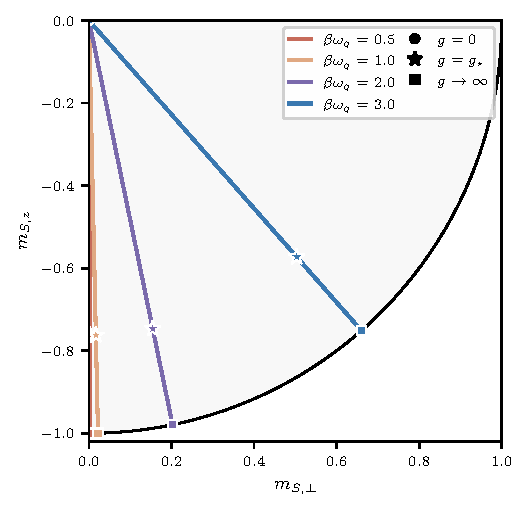
\includegraphics[width=\textwidth]{../figures/hmf_bloch_disk_portrait.pdf}
    \caption{Coupling-plane portrait of the qubit mean-force state.
    \textbf{(a)} Bloch disk cross-section in the coupling plane $(m_x, m_z)
    = (\langle\sigma_x\rangle, \langle\sigma_z\rangle)$ for $\theta = 3\pi/8$
    (Ohmic bath, $\alpha=1$, $\omega_c = 5\,\omega_q$).  Each colored curve
    shows the trajectory of the exact mean-force Bloch vector $\mathbf{r}$ as $\chi$ increases
    from zero.  Filled circles mark $\chi=0$ (bare thermal state on the
    $-\hat{\mathbf{n}}_s$ axis); stars mark the crossover $\chi=1$; squares
    mark the large-$\chi$ attractor.  The gray arrow indicates the bare coupling
    direction $\hat{\mathbf{f}}$; the actual attractor lies in a different,
    temperature-dependent direction set by the bath-channel anisotropy
    (Sec.~\ref{sec:numerical_results_v2}).
    \textbf{(b)} Bloch radius $r = |\mathbf{r}|$ vs.\ $\chi$
    for the same temperatures.  Dotted horizontals show the bare thermal purity
    $r_{\rm bare} = \tanh(\beta\omega_q/2)$.  Every trajectory lies strictly
    above its own $r_{\rm bare}$ (Eq.~\eqref{eq:purity_bound}): bath coupling
    always increases purity regardless of temperature.  The gain is largest at
    high temperature (red), where the bare state is near the maximally-mixed
    center of the disk.}
    \label{fig:bloch_disk_portrait}
\end{figure*}

\subsection{Weak- and strong-coupling limits}
\label{subsec:limits}

The weak- and strong-coupling limits are controlled by the single crossover
variable $\chi$.  For $\chi\ll 1$,
\begin{equation}
    \gamma(\chi)=1-\frac{\chi^2}{3}+O(\chi^4),
    \qquad
    \mathbf u=\mathbf h_{\mathrm{eff}}+O(\chi^3),
\end{equation}
and the Bloch vector expands as
\begin{equation}
    \mathbf r
    =
    -\tanh a\,\hat{\mathbf{n}}_s
    + \operatorname{sech}a\,\mathbf h_{\mathrm{eff},\perp}
    + \operatorname{sech}^2a\,h_{\parallel}\,\hat{\mathbf{n}}_s
    + O(\chi^2).
    \label{eq:bloch_weak}
\end{equation}
Both the induced coherence ($\propto \mathbf h_{\mathrm{eff},\perp}$) and the
longitudinal population correction ($\propto h_\parallel$) are $O(\chi^2)$.

For $\chi\gg 1$,
\begin{equation}
    \gamma(\chi)\sim \chi^{-1},
    \qquad
    \mathbf u=\tanh\chi\,\hat{\mathbf h}_{\mathrm{eff}}
    \to \hat{\mathbf h}_{\mathrm{eff}}+O(e^{-2\chi}),
\end{equation}
so the dependence on the \emph{magnitude} of $\mathbf h_{\mathrm{eff}}$
saturates and only its direction survives:
\begin{equation}
\begin{split}
    \mathbf r
    &\to
    \frac{
        \hat{\mathbf h}_{\mathrm{eff},\perp}
        + \left(\hat h_{\parallel}\cosh a-\sinh a\right)\hat{\mathbf{n}}_s
    }{
        \cosh a-\hat h_{\parallel}\sinh a
    }
    \qquad (\chi\gg 1,\; a\ \text{fixed}).
\end{split}
    \label{eq:bloch_strong}
\end{equation}
The crossover is a smooth, exact interpolation controlled by $\chi$: small
$\chi$ gives linear response around the bare thermal axis
$-\tanh a\,\hat{\mathbf{n}}_s$, while large $\chi$ locks the state to a
temperature-dependent direction determined by the competition between
$\hat{\mathbf{n}}_s$ and $\hat{\mathbf h}_{\mathrm{eff}}$.

\subsection{Relation to weak- and ultrastrong-coupling mean-force results}
\label{subsec:qubit_relation_to_limits}

It is useful to make explicit how the exact qubit geometry derived above relates
to the weak- and ultrastrong-coupling mean-force Gibbs (MFG) results in the
literature, in particular the qubit limit discussed by Cresser and Anders.  Their
central ultrastrong statement is a \emph{basis-selection} result: as the coupling
scale $\lambda\to\infty$, the MFG state becomes diagonal in the eigenbasis of
the coupling operator $X$, rather than in the bare Hamiltonian basis
$H_Q$~\cite{cresserWeakUltrastrongCoupling2021a}.  For a qubit with coupling axis $\hat{\mathbf
f}$ and bare Hamiltonian axis $\hat{\mathbf{n}}_s$, this yields a limiting state whose
Bloch vector points along $\hat{\mathbf f}$ (with a temperature-dependent
magnitude set by the projected bare splitting).

Our exact Gaussian qubit solution is not in contradiction with that result, but
it resolves a different structure. The qubit geometry obtained here proceeds in
two distinct steps:
\begin{equation}
(\hat{\mathbf{n}}_s,\hat{\mathbf f};\text{bath}) \;\longmapsto\; \mathbf h_{\mathrm{eff}}
\;\longmapsto\; \mathbf r .
\end{equation}
The first map constructs a \emph{bath-dressed influence direction} through the
symmetrised exponent, Eq.~\eqref{eq:heff_def}, which is explicitly anisotropic
in the pair of directions $\{\hat{\mathbf f}_\perp,\hat{\mathbf{n}}_s\}$, with separate
weights carried by the non-resonant and resonant bath channels.  The second map
then combines this dressed influence with the bare Gibbs factor $\Pi$ to
produce the final Bloch vector $\mathbf r$.  The bath does not merely rescale
$\hat{\mathbf f}$; it remaps the coupling geometry relative to the system axis before
thermal recombination.

Rewriting $\mathbf h_{\mathrm{eff}}$ in the coupling-adapted frame with
$c\equiv \cos\theta$, $s\equiv \sin\theta$:
\begin{equation}
\mathbf h_{\mathrm{eff}}
=
s^2 c\,(\Sigma_z - \Sigma_\perp)\,\hat{\mathbf f}
+
s\,(\Sigma_\perp c + \Sigma_z s^2)\,\hat{\mathbf n}^{(f)}_\perp ,
\label{eq:heff_coupling_frame}
\end{equation}
where $\hat{\mathbf n}^{(f)}_\perp \equiv (\hat{\mathbf{n}}_s-c\hat{\mathbf f})/s$.
The coupling-axis ultrastrong geometry of Cresser--Anders is recovered only when $\mathbf h_{\mathrm{eff}}$ aligns with $\hat{\mathbf f}$. From Eq.~\eqref{eq:heff_coupling_frame}, this requires the resonant and non-resonant bath channels to satisfy a specific ratio that compensates for the coupling's geometric anisotropy:
\begin{equation}
\frac{\Sigma_z}{\Sigma_\perp} = -\frac{c}{s^2}
\label{eq:ultrastrong_alignment_condition}
\end{equation}
(or equivalently $\Sigma_\perp c + \Sigma_z s^2 = 0$).
which is a special condition on the bath parameters. Absent
Eq.~\eqref{eq:ultrastrong_alignment_condition}, the exact Gaussian qubit state
may still enter the strong-coupling crossover (large $\chi$), but approaches a
bath-dressed attractor direction rather than the bare coupling axis itself (see
the squares in Fig.~\ref{fig:bloch_disk_portrait}a).

A useful summary is therefore:
\begin{quote}
The Cresser--Anders ultrastrong theorem identifies the asymptotic \emph{basis}
selected in the singular coupling limit, while the present exact qubit geometry
resolves the \emph{route} to strong coupling in terms of a bath-anisotropic
dressed influence vector built from resonant and non-resonant channels.
\end{quote}
